\documentclass[a4paper,10pt]{article}
\usepackage[utf8]{inputenc}
\usepackage[slovene]{babel}
\usepackage[left=2cm,top=2.3cm,right=2cm,nohead]{geometry}
\usepackage{amsmath}
\usepackage{amsfonts}
\usepackage{amssymb}
\usepackage[pdftex]{graphicx}
\usepackage{subfig}
\usepackage{textcomp}
\usepackage{tikz}
\usetikzlibrary{positioning,shapes,shadows,arrows,calc}

\begin{document}
\begin{titlepage}
  \let\footnotesize\small
  \let\footnoterule\relax
  \let \footnote \thanks
  \null\vfil
  \vskip 60pt
  \begin{center}
    {\LARGE \textbf{Hivemind} \\ Porazdeljeni Quake 2 bot \par}
    \vskip 3em
    {\large
     \lineskip .75em
      \begin{tabular}[t]{c}
        Grega Kešpret \\
        Jernej Kos \\
        Anže Vavpetič
      \end{tabular}\par}
      \vskip 1.5em
    {\large \today \par}
  \end{center}\par
  \vfil\null
\end{titlepage}


\section{Predstavitev in razdelitev problema}

Cilj naše seminarske naloge je bil izdelava skupine avtonomnih botov (agentov), ki so zmožni navigacije po navideznem svetu ter medsebojne komunikacije. Navidezni svet smo si izbrali zaradi lažje izdelave senzorjev, saj se nam pri tem ni bilo potrebno ukvarjati s težavami računalniškega vida, ki sam po sebi predstavlja široko področje.

Da bi se torej izognili tem težavam, smo si za navidezno okolje v katerem bodo agenti delovali izbrali svet Quake II. Razlog za to izbiro je, da je implementacija tega sveta že na voljo in sicer pod odprtokodno licenco. To omogoča boljše razumevanje delovanja in tudi morebitne popravke ter integracijo.

Problem smo razdelili na nekaj ključnih podproblemov, katere je potrebno rešiti, da bo avtonomni agent v takem okolju deloval zadovljivo:
\begin{enumerate}
  \item \textbf{Vmesnik do navideznega sveta} je prvi korak, ki omogoča našemu agentu interakcijo z objekti v svetu in tudi povratno informacijo o rezultatih njegovih akcij.
  
  \item \textbf{Nadzor gibanja} je najnižja komponenta sistema, ki omogoča da se agent premika po svetu. Zadovoljiv nadzor gibanja mora omogočati \textit{reaktivno in samodejno izogibanje oviram} transparentno glede na to kaj zahtevajo višji nivoji. Sem spadajo tudi osnovni senzorji potrebni za pridobitev informacij o geometriji sveta.
  
  \item \textbf{Navigacija po svetu} omogoča agentu, da si zgradi notranjo predstavitev virtualnega sveta okoli njega, ki mu omogoča učinkovito načrtovanje poti v njem.
  
  \item \textbf{Stanja agenta} določajo trenutno obnašanje in cilje agenta na najvišjem nivoju.
  
  \item \textbf{Komunikacija} omogoča da se večje število agentov poveže v skupino, katere člani si lahko izmenjujejo znanje o svetu in ga tako hitreje spoznajo. Komunikacija omogoča tudi sodelovanje med člani skupine ter identifikacijo pripadnosti (nekakšen IFF\footnote{Identification Friend or Foe}) v primeru napadov.
\end{enumerate}

Tekom raziskovanja smo zgradili relativno preprosto ogrodje, ki omogoča implementacijo zgoraj omenjenih delov takšnega sistema. V nadaljevanju bomo najprej predstavili hiter pregled arhitekture ter potem lastnosti vsake komponente. Med razvojem so se nekatere prvotno zamišljene rešitve izkazale kot slabe in primorani smo jih bili zamenjati. Tudi te smo dokumentirali in opisali njihove pomanjkljivosti.

\section{Pregled arhitekture rešitve}

% Shema arhitekture
\begin{center}
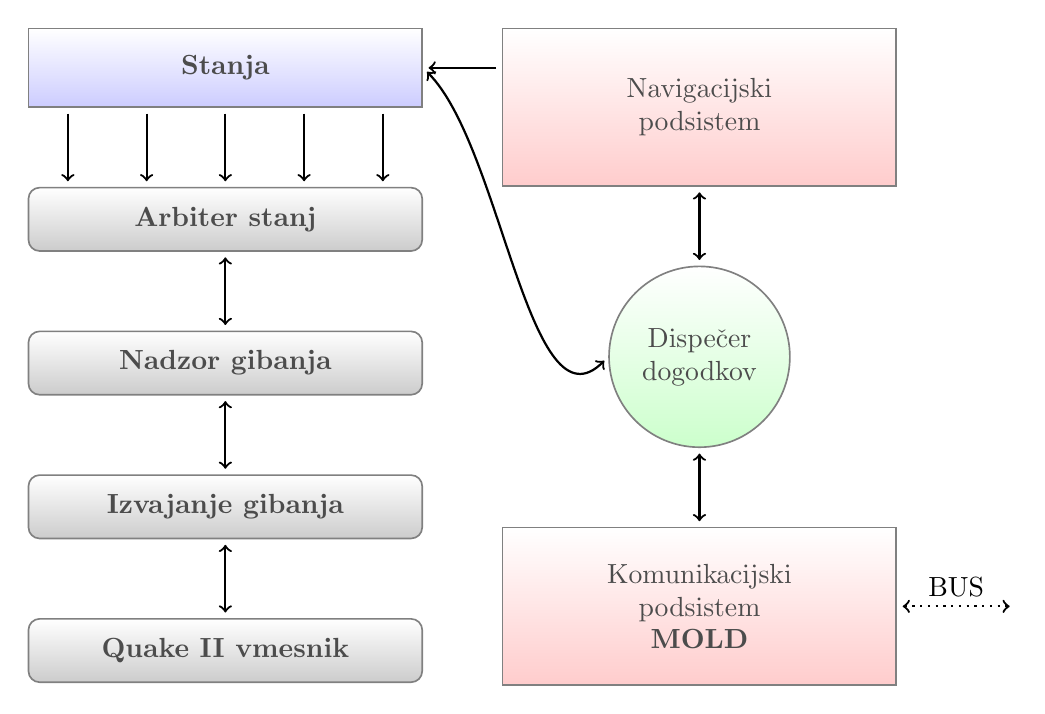
\begin{tikzpicture}[
  semithick,
	node distance=10mm,
	every node/.style={
		text centered
	},
	every path/.style={
		shorten >=2pt,
		shorten <=2pt,
		thick,
		arrows=-stealth'
	},
	colorednode/.style={
		color=black!70,
		rectangle,
		minimum height=6mm,
		minimum width=5cm,
		semithick,
		draw=black!50,
		top color=white,
		bottom color=black!20,
		rounded corners,
		inner sep=7pt
	},
	states/.style={
	  color=black!70,
		rectangle,
		minimum height=1cm,
		minimum width=5cm,
		semithick,
		draw=black!50,
		top color=white,
		bottom color=blue!20,
		inner sep=7pt
	},
	subsystem/.style={
	  color=black!70,
		rectangle,
		minimum height=2cm,
		minimum width=5cm,
		semithick,
		draw=black!50,
		top color=white,
		bottom color=red!20,
		inner sep=7pt
	},
	dispatcher/.style={
	  color=black!70,
		circle,
		minimum height=2cm,
		minimum width=2cm,
		semithick,
		draw=black!50,
		top color=white,
		bottom color=green!20,
		inner sep=7pt
	}
]

  \node (Q2Vmesnik) [colorednode] { \textbf{Quake II vmesnik} };
  \node (IzvajanjeGibanja) [colorednode, above=of Q2Vmesnik] { \textbf{Izvajanje gibanja} };
  \node (NadzorGibanja) [colorednode, above=of IzvajanjeGibanja] { \textbf{Nadzor gibanja} };
  \node (Arbiter) [colorednode, above=of NadzorGibanja] { \textbf{Arbiter stanj} };
  \node (Stanja) [states, above=of Arbiter] { \textbf{Stanja} };
  \node (Navigacija) [subsystem, right=of Stanja, yshift=-5mm] { \shortstack{ Navigacijski \\ podsistem } };
  \node (Dispatcher) [dispatcher, below=of Navigacija] { \shortstack{ Dispečer \\ dogodkov } };
  \node (Komunikacija) [subsystem, below=of Dispatcher] { \shortstack{ Komunikacijski \\ podsistem \\ \textbf{ MOLD } } };
  
  \draw[->] ($ (Stanja.south) - (2cm,0) $) -- ($ (Arbiter.north) - (2cm,0) $);
  \draw[->] ($ (Stanja.south) - (1cm,0) $) -- ($ (Arbiter.north) - (1cm,0) $);
  \draw[->] ($ (Stanja.south) - (0cm,0) $) -- ($ (Arbiter.north) - (0cm,0) $);
  \draw[->] ($ (Stanja.south) + (1cm,0) $) -- ($ (Arbiter.north) + (1cm,0) $);
  \draw[->] ($ (Stanja.south) + (2cm,0) $) -- ($ (Arbiter.north) + (2cm,0) $);
  \draw[<->] (Arbiter) -- (NadzorGibanja);
  \draw[<->] (NadzorGibanja) -- (IzvajanjeGibanja);
  \draw[<->] (IzvajanjeGibanja) -- (Q2Vmesnik);
  
  \draw[->] ($ (Navigacija.west) + (0,5mm) $) -- (Stanja);
  \draw[<->] (Navigacija) -- (Dispatcher);
  \draw[<->] (Dispatcher) -- (Komunikacija);
  \draw[<->] (Stanja.east) .. controls +(1,-1) and +(-1,-1) .. (Dispatcher.west);
  
  \draw[<->,dotted] (Komunikacija.east) -- node[above] {BUS} +(1.5cm,0); 
\end{tikzpicture}
\end{center}

Osnovna arhitektura močno sledi podproblemom, ki smo jih predstavili v uvodu. Posamezne komponente so organizirane kot C++ razredi, povezani preko neposrednih klicev ali pa preko dogodkov.

Celoten sistem je predstavljen s pomočjo centralne komponente imenovane \texttt{Context}. Ta komponenta povezuje vse ostale v celoto in skrbi za uspešno inicializacijo vmesnika do virtualnega sveta, komunikacijskega podsistema, dispečerja dogodkov ipd. Omogoča tudi nekaj osnovnih storitev kot je izpis sporočil za potrebe spremljanja poteka izvajanja programa.

\section{Vmesnik do virtualnega sveta}

Kot naš virtualni svet smo vzeli svet Quake II, ki omogoča dva načina vključitve v sam svet:
\begin{enumerate}
  \item \textbf{UDP/IP povezava odjemalca} se v osnovi obnaša popolnoma enako kot uraden Quake II odjemalec, ki je namenjen večigralstvu. Za to je potrebno razumevanje in implementacija Quake II protokola.
  
  \item \textbf{Integracija v naslovni prostor igre} je v osnovni namenjena t.i. \textit{strežniškim botom} pa tudi najrazličnejšim dodatkom in razširitev igre.
\end{enumerate}

Ker je cilj narediti avtonomne agente, ki niso na nikakršen način priviligirani nad ostalimi igralci, poleg tega pa morajo biti tudi sposobni delovanja iz različnih sistemov IP\footnote{V mrežo povezanih računalnikov} je edina smiselna možnost prva. Zaradi tega je bil prvi korak razumevanje in implementacija Quake II protokola. % TODO

Vendar pa naše ogrodje relativno transparentno podpira tudi drugi način za potrebe pospešene simulacije. Razlogi za to so opisani v enem izmed kasnejših poglavij, ki opisuje \textit{evolucijske umetne nevronske mreže}. Čeprav samega pristopa kasneje nismo uporabili, se je podpora za takšen način simulacije ohranila.

\section{Nadzor gibanja in izogibanje oviram}

\subsection{Senzorji}

\subsection{Nadzorni sistem z EANN}

\subsection{Nadzorni sistem z mehko logiko}

\section{Navigacija po svetu}

\subsection{Statična geometrija iz BSP map}

\subsection{Samodejno učenje topografije}

\subsection{Iskanje poti skozi svet}

\section{Stanja robota}

\subsection{Arbitraža}

\subsection{Reinforcement learning}
% TODO a obstaja kakšen boljši slovenski izraz za RL?

\section{Komunikacija med instancami}

\subsection{MOLD (Message Oriented Lightweight Distributor)}

\subsection{Potek komunikacije}

\section{Možne izboljšave}

\section{Zaključek}

\end{document}

